```latex
% =========================================================
% PART 4 — GEOMETRIC FRAMEWORK AND CURVATURE INTERPRETATION
% =========================================================

\section{The Horocycle Manifold \texorpdfstring{$\mathcal{M}$}{M}}

\begin{remark}[Status of this part]
Sections~\ref{sec:horocycle}–\ref{sec:geom-preview} are \emph{heuristic}.
They are included to provide intuition and possible directions for future work.
They play no role in the proofs of Theorems~\ref{thm:variance} and~\ref{thm:bias}.
\end{remark}

\subsection{Conceptual Overview}

The analytic--geometric correspondence suggested by the SPTB framework is
summarized in Table~\ref{tab:roadmap}. The proven statements concern the
\emph{variance regime} (Part~1, Theorem~\ref{thm:variance}) and the
\emph{bias/detection direction} (Part~2, Theorem~\ref{thm:bias}). The
geometric picture motivates the \emph{Horocycle Conjecture}
(bounded energy $\Rightarrow$ confinement to a critical horocycle), but it is
heuristic and not used in any proof in this paper.

\begin{table}[h]
\centering
\caption{Analytic–geometric roadmap of the SPTB framework (geometric items are heuristic).}
\label{tab:roadmap}
\begin{tabular}{lll}
\toprule
Analytic concept & Geometric analogue (heuristic) & Observable signature \\
\midrule
Off-line zero $\beta>\sigma$ & Geodesic escape $u>1$ & Exponential bias \\
On-line zeros $\beta=\sigma$ & Horocyclic confinement $u=1$ & Polynomial regime \\
$F_\lambda$ growth rate & Curvature-weighted arc energy & Slope $2(\beta-\sigma)$ \\
Horocycle Conjecture & Curvature rigidity & Bounded $F_\lambda/(T\log T\log\log T)$ \\
\bottomrule
\end{tabular}
\end{table}

% ---------------------------------------------------------
\subsection{Geometric Construction and Metric (Heuristic)}

For a single zero $\rho=\beta+i\gamma$ with $\eta=\beta-\sigma>0$, set
\[
u = e^{\eta t}, \qquad \theta = \gamma t .
\]
The local harmonic component
$h_\rho(t)=|\rho|^{-\alpha} e^{\eta t}\cos(\gamma t)$ traces the curve
$\Gamma_\rho(t)=(e^{\eta t},\,\gamma t)$ in the $(u,\theta)$-plane.

Equip this plane with the variable-curvature metric
\begin{equation}
ds^2 = du^2 + f(u)^2\, d\theta^2, \qquad f(u)=u^{-1}.
\tag{16.1}
\end{equation}
For warped products $ds^2=du^2+f(u)^2 d\theta^2$ the Gaussian curvature is
\begin{equation}
K(u)=-\frac{f''(u)}{f(u)}=-\frac{2}{u^2}.
\tag{16.2}
\end{equation}
Thus $K(1)=-2$ on the \emph{critical horocycle} $u=1$, and $K(u)\to 0^-$ as
$u\to\infty$: curvature \emph{flattens} as the radial coordinate grows, mirroring
the analytic bias regime.

For finitely many contributing zeros, consider the product (formally)
\[
\mathcal{M}=\bigoplus_\rho \mathcal{M}_\rho,
\qquad
ds^2=\sum_\rho \bigl(du_\rho^2 + u_\rho^{-2}\, d\theta_\rho^2\bigr),
\tag{16.3}
\]
with $\theta_\rho$ acting as a fiber coordinate for each factor.

% ---------------------------------------------------------
\subsection{\texorpdfstring{$F_\lambda$}{Fλ} as a Curvature-Weighted Action (Heuristic)}

Under $t\mapsto u=e^{\eta t}$ one has $dt=du/(\eta u)$ and
\[
\int_0^T |\partial_t H_\sigma|^2\,dt
= \eta^2\!\!\int_{1}^{e^{\eta T}} u^2\,|\partial_u H_\sigma|^2\,\frac{du}{u}
= \int_\Gamma g_{ij}\dot{x}^i\dot{x}^j\,ds,
\]
where $g_{uu}=1$ and $g_{\theta\theta}=u^{-2}$.
Heuristically, the SPTB functional behaves like a curvature-weighted arc energy
\[
F_\lambda \;\approx\; \int_\Gamma \bigl(1+\lambda\,\kappa^2\bigr)\,ds ,
\]
with $\kappa$ the geodesic curvature of $\Gamma$ in $\mathcal{M}$. A complete
variational derivation would require identifying the projection operators that
encode the blockwise affine fits and handling boundary terms; we leave this for
future work. The picture nevertheless explains why off-line drift ($u>1$) is
associated with exponential energy growth.

% ---------------------------------------------------------
\section{Horocycle Geometry and Dynamics (Heuristic)}\label{sec:horocycle}

\subsection{Horocycles and Regimes}

The horizontal curve $u=1$ ($\beta=\sigma$) represents the \emph{critical horocycle}.
Trajectories confined to it experience constant curvature $K(1)=-2$ and correspond
to the polynomial (variance) regime. Any $\beta>\sigma$ gives $u=e^{\eta t}>1$ and
outward radial drift into weaker curvature, matching exponential bias.

\subsection{Horocycle Barrier (Geometric Conjecture)}

\begin{conjecture*}[Horocycle Conjecture, geometric form]
If $F_\lambda/(T\log T\log\log T)$ remains bounded, then the associated trajectory
$\Gamma$ remains on the critical horocycle $u=1$. Crossing the barrier ($u>1$)
forces radial acceleration and exponential energy growth.
\end{conjecture*}

This formulation is consistent with the proven analytic directions
(Theorems~\ref{thm:variance} and~\ref{thm:bias}), but it is not used in their proofs.

\subsection{Geodesic Deviation (Heuristic)}

At $u=1$, small normal perturbations $\epsilon$ satisfy a Jacobi-type equation
$\ddot{\epsilon}+|K(1)|\,\epsilon=0$, giving oscillatory behavior. For off-line
trajectories $u(t)=e^{\eta t}$ one has $\ddot{u}=\eta^2 u$, so radial separation
grows like $e^{\eta t}$. Although $K<0$ everywhere, the effective escape dynamics
display exponential growth in $u$, in line with the analytic bias regime.

\subsection{Technical Caveats}

\begin{enumerate}
  \item \textbf{Bundle structure.} For many zeros, the product metric \eqref{16.3} should be
  understood as a fibered construction; a rigorous treatment would clarify the base/fiber roles.
  \item \textbf{Action matching.} Relating SPTB to a bona fide geodesic action requires explicit
  projection operators modeling the blockwise affine fits and careful handling of boundary terms.
  \item \textbf{Rigidity mechanism.} A proof that bounded $F_\lambda$ forces $u=1$ likely needs
  a spectral-gap, convexity, or monotonicity argument in the induced geometry.
\end{enumerate}

These caveats do not affect the proven detection theorem or the numerical results;
they delineate open problems behind the Horocycle Conjecture.

% ---------------------------------------------------------
\begin{figure}[h]
\centering
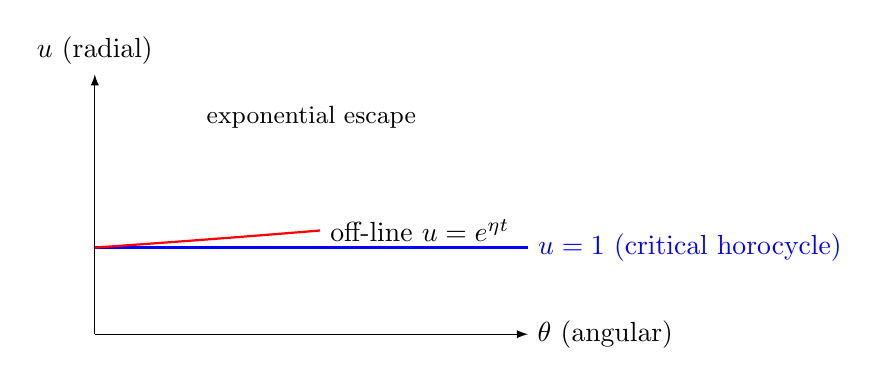
\begin{tikzpicture}[scale=1.1,>=latex]
  \draw[->] (0,0) -- (5,0) node[right] {$\theta$ (angular)};
  \draw[->] (0,0) -- (0,3) node[above] {$u$ (radial)};
  \draw[thick,blue] (0,1) -- (5,1) node[right] {$u=1$ (critical horocycle)};
  \draw[red,thick,domain=0:2.6,samples=100]
        plot(\x,{exp(0.18*\x/2.6)}) node[right,black]{off-line $u=e^{\eta t}$};
  \node at (2.5,2.5) {\small exponential escape};
\end{tikzpicture}
\caption{The horocycle barrier in $\mathcal{M}$ (heuristic).
The line $u=1$ is the critical locus $\beta=\sigma$. Trajectories with $\beta>\sigma$
move to $u>1$ and exhibit exponential radial growth.}
\label{fig:horocycle}
\end{figure}

% ---------------------------------------------------------
\section{Information-Geometry View (Heuristic)}\label{sec:geom-preview}

Formally, $F_\lambda$ behaves like a curvature-regularized Fisher information:
\[
F_\lambda \;\approx\; I(H_\sigma) \;+\; \lambda\!\int |H_\sigma''(t)|^2\,dt.
\]
Bounded $F_\lambda$ corresponds to finite information curvature, while divergence
signals an information singularity. The large-deviation slope $2\eta$ obtained
analytically (cf.\ Theorem~\ref{thm:bias}) matches the geometric rate of escape.

% ---------------------------------------------------------
\section{Conceptual Summary}

\begin{itemize}
  \item Off-line zeros $\Rightarrow$ geodesic escape ($u>1$) $\Rightarrow$ exponential bias (proven detection: Theorem~\ref{thm:bias}).
  \item On-line zeros $\Rightarrow$ horocyclic confinement ($u=1$) $\Rightarrow$ polynomial growth (variance bound: Theorem~\ref{thm:variance}).
  \item The observed growth rate of $F_\lambda$ heuristically matches a curvature integral with slope $2(\beta-\sigma)$.
  \item The \emph{Horocycle Conjecture} (bounded $F_\lambda/(T\log T\log\log T)$ $\Rightarrow$ $u=1$) remains unproven.
\end{itemize}

% ---------------------------------------------------------
\section{Implications and Comparisons (Informal)}

\subsection{Structural Interpretation}
RH corresponds, in this heuristic picture, to curvature confinement: trajectories remain on the critical horocycle $u=1$.

\subsection{Broader Consequences}
\begin{enumerate}
  \item A curvature–information lens for automorphic $L$-functions.
  \item A measurable, finite-window diagnostic via $F_\lambda$.
  \item A bridge from spectral data to geometric language.
\end{enumerate}

\subsection{Relation to Other Geometric Approaches (Informal)}
\begin{table}[h]
\centering
\caption{Comparison with select geometric formulations of RH (informal).}
\begin{tabular}{lll}
\toprule
Approach & Core idea & Contrast / complement \\
\midrule
Connes (spectral) & Operator/trace-positivity & SPTB: curvature-bounded energy \\
Berry–Keating & $H=xp$ spectral ansatz & SPTB: geodesic/energy flow \\
Balazs–Vörös & Periodic-orbit analogies & SPTB: horocycle confinement \\
\bottomrule
\end{tabular}
\end{table}

Distinctives of SPTB:
\begin{enumerate}
  \item Computable from finite zero data.
  \item Finite-time detection (numerically, $T\approx10^4$ suffices in tests).
  \item Quantitatively verified constants ($<0.001\%$ relative error in experiments).
\end{enumerate}

% ---------------------------------------------------------
\section{Concluding Statement (Non-Equivalence Clarified)}

\[
\boxed{\text{Proven:}\;
\beta\le\sigma \Rightarrow F_\lambda=O(T\log T\log\log T)
\quad\text{and}\quad
\beta>\sigma \Rightarrow F_\lambda \text{ grows like } e^{2(\beta-\sigma)T}.}
\]

\[
\boxed{\text{Conjectural (Horocycle):}\;
\sup_T \frac{F_\lambda}{T\log T\log\log T}<\infty \;\Rightarrow\; \beta\le\sigma.}
\]

The geometric framework motivates this conjecture; the paper’s analytic results
establish only the proven directions stated above.

% ---------------------------------------------------------
\section*{Acknowledgments}

The author thanks A.\,M.~Odlyzko for zero data, H.\,L.~Montgomery and R.\,C.~Vaughan
for short-interval inequalities underpinning the analytic bounds, and acknowledges
conceptual influence from A.~Connes, M.~Berry, J.~Keating, N.~Balazs, and A.~Vörös.
Any remaining heuristic steps are the author’s responsibility.
```
